\section{Potenziale Elettrico}
\subsection{Energia potenziale elettrica}

La forza elettrica agente su un aparticella di prova è:
\begin{equation*}
    \vec{F} = q_0\vec{E}
\end{equation*}

\begin{figure}[H]
    \centering
    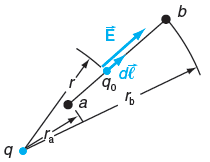
\includegraphics[width=0.2\linewidth]{imgs/9 - potenziale.png}
    \label{fig:potenziale}
    \caption{Esempio di potenziale con sfera}
\end{figure}
\begin{equation}
    \int_a^b{\vec{F}\cdot d\vec{l}} = 
    Edl\cos{90^{\circ}} = 0
\end{equation}
Dove la formula del campo elettrico è:
\begin{equation*}
    \vec{E} = \frac{q}{4\pi\epsilon_0 r^2}\hat{r}
\end{equation*}

La formula generale per calcolare il lavoro è la seguente:
\begin{equation}
    \int_a^b{\vec{F}\cdot d\vec{l}} = 
    \frac{q_0q}{4\pi\epsilon_0}
    \Bigg(\frac{1}{r_a}-\frac{1}{r_b}\Bigg)
\end{equation}

Il lavoro compiuto da una forza elettrica è indipendente dalla traiettroia.

\begin{equation}
    U_b - U_a =
    - \int_a^b{\vec{F}\cdot d\vec{l}} =
    \frac{q_0q}{4\pi\epsilon_0}
    \Bigg(\frac{1}{r_b}-\frac{1}{r_a}\Bigg)
\end{equation}
Nota che ho cambiato b con a per il segno negativo.

\subsubsection{Energia con tante cariche puntiformi}
Avendo varie cariche puntiformi, si sommano vettorialmente i loro valori.
\begin{equation*}
    \vec{F} = q_0\vec{E} = q_0\Bigg(\sum_i{\vec{E_i}}\Bigg)
\end{equation*}

\subsubsection{Formula generale}
\begin{equation}
    U = \frac{q_0}{4\pi\epsilon_0}\Bigg(\sum_i\frac{q_i}{r_i}\Bigg)
\end{equation}

\subsection{Potenziale elettrico}
\begin{equation}
    V = \frac{U}{q_0}
\end{equation}
Il potenziale prodotto in un punto P da una distribuzione di cariche:

\begin{equation}
    V = \frac{1}{4\pi\epsilon_0}\Bigg(\sum_i\frac{q_i}{r_i}\Bigg)
\end{equation}

\subsection{Elettronvolt}
\begin{equation*}
    1eV = (1.6 \times 10^{-19}C)(1V) = 1.6\times 10^{-19}J
\end{equation*}
1 eV é l'energia guadagnata da un elettrone attraverso una differenza
di potenziale di 1 V.

\subsection{Potenziale prodotto da distribuzione continua di carica}
Con il passaggio al limite, la sommatoria diventa un integrale.
\begin{equation}
    V = \frac{1}{4\pi\epsilon_0}\int\frac{dq}{r}
\end{equation}

\subsection{Differenza di potenziale}
\begin{equation}
    V_b - V_a = -\int_a^b{\vec{E}\cdot d\vec{l}}
\end{equation}

\subsection{Campo in funzione del potenziale}
\begin{equation}
    \vec{E} =
    - \Bigg(
        \frac{\delta V}{\delta x}\hat{x} +
        \frac{\delta V}{\delta y}\hat{y} +
        \frac{\delta V}{\delta z}\hat{z}
    \Bigg)
\end{equation}


\subsection{Potenziale e campo elettrico}
Potenziale e campo elettrico sono direttamente correlati:
\begin{itemize}
    \item entrambi possono essere determinati dalla distribuzione di cariche
    \item possono essere determinati a partire dall'altro
\end{itemize}

La dimensione del campo elettrico è $[\frac{V}{m}]$ o $[\frac{N}{C}]$.

\subsection{Campo elettrostatico}
Il campo elettrostatico è conservativo quando la sua cortocircuitazione è nulla.
\begin{equation*}
    \oint{\vec{E}\cdot d\vec{l}} = 0
\end{equation*}
E si può usare la fromula sia su una line ache su un volume ed una superficie,
se si usa la variazione di suerficie si usa un doppio integrale e
per il volume si usa un tripolo integrale.

\subsection{Superficie equipotenziali}
Superfici che hanno lo stesso potenziale
(come una sfera, armatura di un condensatore).

\subsection{Conduttori}
Dentro ad un conduttore, il campo E è nullo, mentre il potenziale è costante.
All'esterno entrambi decadono con l'aumetare della distanza(il campo decade più in fretta).

\begin{figure}[H]
    \centering
    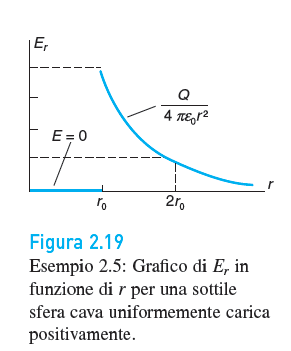
\includegraphics[width=0.25\linewidth]{imgs/10 - campo vs potenziale.png}
    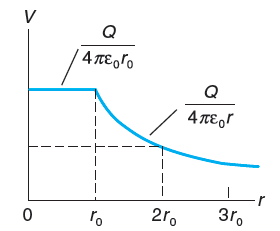
\includegraphics[width=0.25\linewidth]{imgs/11 - campo vs potenziale2.png}
    \caption{Potenziale Vs Campo}
    \label{fig:potenziale_vs_campo}
\end{figure}

\subsection{Rigidità dielettrica}
La rigidità dielettrica è il massimo campo applicabile ad un isolante prima che questo
smetta di isolare e permetta il passaggio delle cariche.
Esempio: fulmini(l'aria isola finchè il campo elettrico non è troppo grande
e tenta di scaricare verso terra).